\chapter{Running jobs with input/output data}
\label{ch:running-jobs-with-input-output-data}

You have now learned how to start a batch job and how to start an interactive
session.  The next question is how to deal with input and output files, where
your standard output and error messages will go to and where that you can
collect your results.

\section{The current directory and output and error files}

\subsection{Default file names}

First go to the directory:

\begin{prompt}
%\shellcmd{cd ~/\exampledir{}}%
\end{prompt}

List and check the contents with:

\begin{prompt}
%\shellcmd{ls -l}%
total 2304
-rwxrwxr-x 1 %\userid{}%  682 Sep 13 11:34 file1.py
-rw-rw-r-- 1 %\userid{}%  212 Sep 13 11:54 file1a.pbs
-rw-rw-r-- 1 %\userid{}%  994 Sep 13 11:53 file1b.pbs
-rw-rw-r-- 1 %\userid{}%  994 Sep 13 11:53 file1c.pbs
-rw-r--r-- 1 %\userid{}% 1393 Sep 13 10:41 file2.pbs
-rwxrwxr-x 1 %\userid{}% 2393 Sep 13 10:40 file2.py
-rw-r--r-- 1 %\userid{}% 1393 Sep 13 10:41 file3.pbs
-rwxrwxr-x 1 %\userid{}% 2393 Sep 13 10:40 file3.py
\end{prompt}

Now, let us inspect the contents of the first executable (which is just a
Python script with execute permission).

\examplecode{Python}{file1.py}

The code of the Python script, is self explanatory:
\begin{enumerate}
\item  In step 1, we write something to the file \texttt{hello.txt} in the current directory.
\item  In step 2, we write some text to stdout.
\item  In step 3, we write to stderr.
\end{enumerate}

Check the contents of the first job script:

\examplecode{bash}{file1a.pbs}

You'll see that there are NO specific PBS directives for the placement of the output files. All output files are
just written to the standard paths.

Submit it:

\begin{prompt}
%\shellcmd{qsub file1a.pbs}%
\end{prompt}

After the job has finished, inspect the local directory again, i.e., the
directory where you executed the \emph{qsub} command:

\begin{prompt}
%\shellcmd{ls -l}%
total 3072
-rw-rw-r-- 1 %\userid{}%   90 Sep 13 13:13 Hello.txt
-rwxrwxr-x 1 %\userid{}%  693 Sep 13 13:03 file1.py*
-rw-rw-r-- 1 %\userid{}%  229 Sep 13 13:01 file1a.pbs
-rw------- 1 %\userid{}%   91 Sep 13 13:13 file1a.pbs.e%\jobnumber{}%
-rw------- 1 %\userid{}%  105 Sep 13 13:13 file1a.pbs.o%\jobnumber{}%
-rw-rw-r-- 1 %\userid{}%  143 Sep 13 13:07 file1b.pbs
-rw-rw-r-- 1 %\userid{}%  177 Sep 13 13:06 file1c.pbs
-rw-r--r-- 1 %\userid{}% 1393 Sep 13 10:41 file2.pbs
-rwxrwxr-x 1 %\userid{}% 2393 Sep 13 10:40 file2.py*
-rw-r--r-- 1 %\userid{}% 1393 Sep 13 10:41 file3.pbs
-rwxrwxr-x 1 %\userid{}% 2393 Sep 13 10:40 file3.py*
\end{prompt}

Some observations:
\begin{enumerate}
\item The file \texttt{Hello.txt} was created in the current directory.
\item The file \texttt{file1a.pbs.o\jobnumber} contains all the text that was written to the standard output stream (``stdout'').
\item The file \texttt{file1a.pbs.e\jobnumber} contains all the text that was written to the standard error stream (``stderr'').
\end{enumerate}

Inspect their contents \dots\ and remove the files

\begin{prompt}
%\shellcmd{cat Hello.txt}%
%\shellcmd{cat file1a.pbs.o\jobnumber{}}%
%\shellcmd{cat file1a.pbs.e\jobnumber{}}%
%\shellcmd{rm Hello.txt file1a.pbs.o\jobnumber{} file1a.pbs.e\jobnumber{}}%
\end{prompt}

\begin{tip}
Type ``\texttt{cat H}'' and press the \keys{TAB} button, and it will
\strong{expand} into full filename \texttt{Hello.txt}.
\end{tip}

\subsection{Filenames using the name of the job}

Check the contents of the job script and execute it.

\examplecode{bash}{file1b.pbs}

\begin{prompt}
%\shellcmd{qsub file1b.pbs}%
\end{prompt}

Inspect the contents again \dots\ and remove the generated files:

\begin{prompt}
%\shellcmd{ls}%
Hello.txt  file1a.pbs  file1c.pbs  file2.pbs  file3.pbs  my_serial_job.e%\jobnumber{}%
file1.py*  file1b.pbs  file2.py*   file3.py*  my_serial_job.o%\jobnumber{}%
%\shellcmd{rm Hello.txt my\_serial\_job.*}%
\end{prompt}

Here, the option ``\texttt{-N}'' was used to explicitly assign a name to the job.  This
overwrote the JOBNAME variable, and resulted in a different name for the
\emph{stdout} and \emph{stderr} files. This name is also shown in the
second column of the ``\texttt{qstat}'' command. If no name is provided, it defaults to
the name of the job script.

\subsection{User-defined file names}

You can also specify the name of \emph{stdout} and \emph{stderr} files
explicitly by adding two lines in the job script, as in our third example:

\examplecode{bash}{file1c.pbs}

\begin{prompt}
%\shellcmd{qsub file1c.pbs}%
%\shellcmd{ls}%
\end{prompt}

\section{Where to store your data on the \hpc}
\hypertarget{where-to-store-data}{}

The \hpc cluster offers their users several locations to store their data. Most
of the data will reside on the shared storage system, but all compute nodes
also have their own (small) local disk.

\subsection{Pre-defined user directories}
\label{subsec:predefined-user-directories}

Three different pre-defined user directories are available, where each
directory has been created for different purposes. The best place to store your
data depends on the purpose, but also the size and type of usage of the data.

The following locations are available:

\begin{tabular}{|p{\dimexpr 0.35\textwidth-2\tabcolsep}|p{\dimexpr 0.65\textwidth-2\tabcolsep}|} \hline
\strong{Variable} & \strong{Description} \\ \hline\hline
\multicolumn{2}{|l|}{\hspace*{2cm}\emph{Long-term storage} slow filesystem, intended for smaller files} \\ \hline
\$VSC\_HOME            & For your configuration files and other small files, see \S\ref{subsec:home-directory}. \newline
                         The default directory is /user/\sitename/xxx/$<$vsc-account$>$.
                         The same file system is accessible from all sites, i.e., you'll see the same contents in \$VSC\_HOME on all sites. \\ \hline
\$VSC\_DATA            & A bigger ``workspace'', for \strong{datasets}, results, logfiles, etc. see \S\ref{subsec:data-directory}. \newline
                         The default directory is /data/\sitename/xxx/$<$vsc-account$>$.
                         The same file system is accessible from all sites. \\ \hline\hline
\multicolumn{2}{|l|}{\hspace*{2cm}\emph{Fast temporary storage}} \\ \hline
\$VSC\_SCRATCH\_NODE   & For \strong{temporary} or transient data on the local compute node, where fast access is important; see \S\ref{subsec:scratch-directory}. \newline
                         This space that is available per node. The default directory is /tmp.
                         On different nodes, you'll see different content. \\ \hline
\$VSC\_SCRATCH         & For \strong{temporary} or transient data that has to be accessible from all nodes of a cluster (including the login nodes) \newline
                         The default directory is /scratch/\sitename/xxx/$<$vsc-account$>$
                         This directory is cluster- or site-specific: On different sites, and sometimes on different clusters on the same site, you'll get a different directory with different content. \\ \hline
\$VSC\_SCRATCH\_SITE   & Currently the same as \$VSC\_SCRATCH, but could be used for a scratch space
                         shared across all clusters at a site in the future. See \S\ref{subsec:scratch-directory}. \\ \hline
\$VSC\_SCRATCH\_GLOBAL & Currently the same as \$VSC\_SCRATCH, but could be used for a scratch space
                         shared across all clusters of the VSC in the future. See \S\ref{subsec:scratch-directory}. \\ \hline
\ifgent
\$VSC\_SCRATCH\_CLUSTER & The scratch filesystem closest to this cluster.\\ \hline
\$VSC\_SCRATCH\_PHANPY  & A separate (smaller) shared scratch filesystem, powered by SSDs. This scratch filesystem is intended for very I/O-intensive workloads.\\ \hline
\fi
\end{tabular}

% Integrated this text in the tables above as it could be misunderstood that
% you'd see the same content on all sites/clusters/nodes.
%These pre-defined directories are mounted on each compute node, so it does not
%matter where your job will actually be executed; all your data is always
%accessible via these directories.

Since these directories are not necessarily mounted on the same locations over
all sites, you should always (try to) use the environment variables that have
been created.

We ellaborate more on the specific function of these locations in the following
sections.

\ifgent
Note: \lstinline|$VSC_SCRATCH_KYUKON| and \lstinline|$VSC_SCRATCH| are the same directories
("kyukon" is the name of the storage cluster where the default shared scratch filesystem is hosted).

For documentation about VO directories, see \autoref{subsec:vo-directories}.
\fi

\subsection{Your home directory (\$VSC\_HOME)\label{subsec:home-directory}}

Your home directory is where you arrive by default when you login to the
cluster. Your shell refers to it as ``\tilde'' (tilde), and its absolute path is also
stored in the environment variable \$VSC\_HOME. Your home directory is shared across
all clusters of the VSC.

The data stored here should be relatively small (e.g., no files or directories
larger than a few megabytes), and preferably should only contain configuration
files.
Note that various kinds of configuration files are also stored
here, e.g., by MATLAB, Eclipse, \ldots

The operating system also creates a few files and folders here to manage your
account. Examples are:

\begin{tabular}{|p{\dimexpr 0.2\textwidth-2\tabcolsep}|p{\dimexpr 0.8\textwidth-2\tabcolsep}|} \hline
\textbf{File or Directory} & \textbf{Description} \\ \hline
.ssh/                      & This directory contains some files necessary for you to login to the cluster and to submit jobs on the cluster. Do not remove them, and do not alter anything if you don't know what you are doing! \\ \hline
.bash\_profile             & When you login (type username and password) remotely via ssh, .bash\_profile is executed to configure your shell before the initial command prompt. \\ \hline
% It's a bad idea to advise users to do 'module load' commands in .bashrc, since this will inevitably result in module conflicts. Removed it.
.bashrc                    & This script is executed every time you start a session on the cluster: when you login to the cluster and when a job starts. \\ \hline
.bash\_history             & This file contains the commands you typed at your shell prompt, in case you need them again. \\ \hline
\end{tabular}

\ifgent
% we don't auto create these files in gent
\else
Furthermore, we have initially created some files/directories there (tutorial,
docs,  examples, examples.pbs) that accompany  this manual and allow you to
easily execute the provided examples.
\fi

\subsection{Your data directory (\$VSC\_DATA)\label{subsec:data-directory}}

In this directory you can store all other data that you need for longer terms
(such as the results of previous jobs, \ldots). It is a good place for, e.g.,
storing big files like genome data.

The environment variable pointing to this directory is \$VSC\_DATA.
This volume is shared across all
clusters of the VSC. There are however no guarantees about the
speed you will achieve on this volume. For guaranteed fast performance and very heavy I/O,
you should use the scratch space instead.
\ifgent
If you are running out of quota on your \$VSC\_DATA filesystem you can
request a VO. See \autoref{sec:virtual-organisations} on how to do this.
\fi

\subsection{Your scratch space (\$VSC\_SCRATCH)\label{subsec:scratch-directory}}

To enable quick writing from your job, a few extra file systems are available
on the compute nodes. These extra file systems are called scratch folders, and can
be used for storage of temporary and/or transient data (temporary results,
anything you just need during your job, or your batch of jobs).

You should remove any data from these systems after your processing them has
finished. There are no guarantees about the time your data will be stored on
this system, and we plan to clean these automatically on a regular base. The
maximum allowed age of files on these scratch file systems depends on the type
of scratch, and can be anywhere between a day and a few weeks. We don't
guarantee that these policies remain forever, and may change them if this seems
necessary for the healthy operation of the cluster.

Each type of scratch has its own use:

\begin{description}
\item[Node scratch (\$VSC\_SCRATCH\_NODE).]
Every node has its own scratch space, which is completely separated from the other nodes.
On some clusters, it will be on a local disk in the node, while on other
clusters it will be emulated through another file server. In many cases,
it will be significantly slower than the cluster scratch as it typically
consists of just a single disk.
Some \strong{drawbacks} are that the storage
can only be accessed on that particular node and that the capacity is often very limited (e.g., 100 GB).
The performance will depend a lot on the particular implementation in the cluster. In many cases,
it will be significantly slower than the cluster scratch as it typically
consists of just a single disk. However, if that disk is local to the node
(as on most clusters), the performance will not depend on what others are
doing on the cluster.
\item[Cluster scratch (\$VSC\_SCRATCH).]
To allow a job running on multiple nodes (or multiple jobs running on
separate nodes) to share data as files, every node of the cluster
(including the login nodes) has access to this shared scratch directory.
Just like the home and data directories, every user has its own scratch
directory. Because this scratch is also available from the login nodes, you
could manually copy results to your data directory after your job has
ended. Also, this type of scratch is usually implemented by running tens or
hundreds of disks in parallel on a powerful file server with fast connection
to all the cluster nodes and therefore is often the fastest file system
available on a cluster. \\
You may not get the same file system on different clusters, i.e., you
may see different content on different clusters at the same intitute.
\ifantwerpen
  At the time of writing, the cluster scratch space is shared between both clusters
  at the \university. This may change again in the future when storage gets
  updated.
\fi
\item[Site scratch (\$VSC\_SCRATCH\_SITE).]
At the time of writing, the site scratch is just the same
volume as the cluster scratch, and thus contains the same data.
In the future it may point to a different scratch file system
that is available across all clusters at a particular site, which is in
fact the case for the cluster scratch on some sites.
\item[Global scratch (\$VSC\_SCRATCH\_GLOBAL).]
At the time of writing, the global scratch is just the same
volume as the cluster scratch, and thus contains the same data.
In the future it may point to a scratch file system
that is available across all clusters of the VSC, but at the moment
of writing there are no plans to provide this.
\end{description}

\subsection{Pre-defined quotas}
\label{subsec:predfined-quotas}
\hypertarget{predefined-quotas}{}

\strong{Quota} is enabled on these directories, which means that the amount of
data you can store there is limited. This holds for both the total size of all
files as well as the total number of files that can be stored. The system works
with a soft quota and a hard quota. You can temporarily exceed the soft quota,
but you can never exceed the hard quota. The user will get warnings as soon as
he exceeds the soft quota.


\ifgent
To see your current quota usage you can run the ``\emph{show\_quota}``` script
on the \hpcInfra.

\begin{prompt}
bash-4.1\$ show_quota
User quota:
VSC_HOME: used 1.08 GiB (37%\%%) quota 2.85 GiB (3 GiB hard limit)
VSC_DATA_VO: used 8.16 MiB (0%\%%) quota 1.62 TiB (1.71 TiB hard limit)
VSC_DATA: used 0 B (0%\%%) quota 23.8 GiB (25 GiB hard limit)
VSC_SCRATCH_GULPIN_VO: used 41.3 GiB (1%\%%) quota 2.32 TiB (2.44 TiB hard limit)
VSC_SCRATCH_GULPIN: used 7.78 MiB (0%\%%) quota 23.8 GiB (25 GiB hard limit)
VSC_SCRATCH_DELCATTY_VO: used 340 GiB (7%\%%) quota 4.52 TiB (4.76 TiB hard limit)
VSC_SCRATCH_DELCATTY: used 11.4 GiB (47%\%%) quota 23.8 GiB (25 GiB hard limit)
\end{prompt}

You can also visit the account page (\url{https://account.vscentrum.be}
to see a list of your current quota and
VO moderators can see a list of VO quota usage per member of their VO.
\else
The amount of data (called ``\emph{Block Limits}'') that is currently in use
by the user (``\emph{KB}''), the soft limits (``\emph{quota}'') and the
hard limits (``\emph{limit''}) for all 3 file-systems are always displayed
when a user connects to the \hpc.

 Whith regards to the \emph{file limits}, the number of files in use
 (``\emph{files}''), its soft limit (``\emph{quota}'') and its hard limit
 (``\emph{limit}'') for the 3 file-systems are also displayed.

\begin{prompt}
----------------------------------------------------------
Your quota is:

                   Block Limits
   Filesystem         KB      quota      limit    grace
   home           177920    3145728    3461120     none
   data         17707776   26214400   28835840     none
   scratch        371520   26214400   28835840     none

                File Limits
   Filesystem      files      quota      limit    grace
   home              671      20000      25000     none
   data           103079     100000     150000  expired
   scratch          2214     100000     150000     none

----------------------------------------------------------
\end{prompt}

Make sure to regularly check these numbers at log-in!
\fi  % end \ifgent \else

The rules are:
\begin{enumerate}
\item  You will only receive a warning when you have reached the soft limit of either quota.
\item  You \emph{will} start losing data and get I/O errors when you reach the hard limit. In this
  case, data loss will occur  since nothing can be written anymore (this holds
  both for new files as well as for existing files), until you free up
  some space by removing some files. Also note that you \emph{will not} be
  warned when data loss occurs, so keep an eye open for the general quota
  warnings!
\item  The same holds for running jobs that need to write files: when you reach
  your hard quota, jobs will crash.
\end{enumerate}

We do realise that quota are often observed as a nuisance by users, especially if you're running low on it.
However, it is an essential feature of a shared infrastructure. Quota ensure that a single user cannot
accidentally take a cluster down (and break other user's jobs) by filling up the available disk space.
And they help to guarantee a fair use of all available resources for all users. Quota also help to ensure
that each folder is used for its intended purpose.

%% I suggest to delete the following section as it contains nothing new.
%\subsection{Local data}

% One could also opt to use some local disk-space on the compute node itself.

% The \strong{advantage} is that this local disk will perform the best for disk-I/O intensive applications.  The \strong{drawback} is that those disks are limited in size (e.g., approx.\ 100 GB depending on the node) and that these disks are not visible from outside.

% But it is for sure useful when you are working with temporary output data in a sequential flow of an application.

% You'll best use the ``/tmp'' directory, which can be accessed via the \$VSC\_SCRATCH\_NODE environment variable.

% \begin{prompt}
% %\shellcmd{echo \$VSC\_SCRATCH\_NODE}%
% /tmp
% \end{prompt}

\section{Writing Output files}

\begin{tip}
Find the code of the exercises in ``\texttt{\tilde/\exampledir}''
\end{tip}

In the next exercise, you will generate a file in the \$VSC\_SCRATCH directory.
In order to generate some CPU- and disk-I/O load, we will

\begin{enumerate}
\item  take a random integer between 1 and 2000 and calculate all primes up to that limit;
\item  repeat this action 30.000 times;
\item  write the output to the ``\texttt{primes\_1.txt}'' output file in the \$VSC\_SCRATCH-directory.
\end{enumerate}

Check the Python and the PBS file, and submit the job: Remember that this is
already a more serious (disk-I/O and computational intensive) job, which takes
approximately 3 minutes on the \hpc.

\begin{prompt}
%\shellcmd{cat file2.py}%
%\shellcmd{cat file2.pbs}%
%\shellcmd{qsub file2.pbs}%
%\shellcmd{qstat}%
%\shellcmd{ls -l}%
%\shellcmd{echo \$VSC\_SCRATCH}%
%\shellcmd{ls -l \$VSC\_SCRATCH}%
%\shellcmd{more \$VSC\_SCRATCH/primes\_1.txt}%
\end{prompt}

\section{Reading Input files}

\begin{tip}
Find the code of the exercise ``\texttt{file3.py}'' in

% Line break because the line is too long.
``\texttt{\tilde/\exampledir}''.
\end{tip}

In this exercise, you will
\begin{enumerate}
\item  Generate the file ``\texttt{primes\_1.txt}'' again as in the previous exercise;
\item  open the this file;
\item  read it line by line;
\item  calculate the average of primes in the line;
\item  count the number of primes found per line;
\item  write it to the ``\texttt{primes\_2.txt}'' output file in the \$VSC\_SCRATCH-directory.
\end{enumerate}

Check the Python and the PBS file, and submit the job:

\begin{prompt}
%\shellcmd{cat file3.py}%
%\shellcmd{cat file3.pbs}%
%\shellcmd{qsub file3.pbs}%
%\shellcmd{qstat}%
%\shellcmd{ls -l}%
%\shellcmd{more \$VSC\_SCRATCH/primes\_2.txt}%
%\dots{}%
\end{prompt}

\section{How much disk space do I get?}
\label{sect:how-much-disk-space-do-i-get}

\subsection{Quota}

The available disk space on the \hpc is limited. The actual disk capacity,
shared by all users, can be found on the ``Available hardware'' page on the
website.
(\url{https://www.vscentrum.be/infrastructure/hardware})
As explained in \S\ref{subsec:predfined-quotas}, this implies
that there are also limits
\begin{enumerate}
\item  to the amount of disk space; and
\item  to the number of files
\end{enumerate}

that can be made available to each individual \hpc user.

The quota of disk space and number of files for each \hpc user is:

\ifantwerpen
\begin{tabular}{|p{0.7in}|r|r|} \hline
\strong{Volume} & \strong{Max.\ disk space} & \strong{Max.\ \# Files} \\ \hline
HOME            & 3 GB                      & 20000                  \\ \hline
DATA            & 25 GB                     & 100000                 \\ \hline
SCRATCH         & 25 GB                     & 100000                 \\ \hline
\end{tabular}
\fi %ENDIF \ifantwerpen
\ifgent
\begin{tabular}{|p{0.7in}|r|r|} \hline
\strong{Volume} & \strong{Max.\ disk space} & \strong{Max.\ \# Files} \\ \hline
HOME            & 3 GB                      & 20000                   \\ \hline
DATA            & 25 GB                     & 100000                  \\ \hline
SCRATCH         & 25 GB                     & 100000                  \\ \hline
\end{tabular}
\fi %ENDIF \ifgent

\begin{tip}
The first action to take when you have exceeded your quota is
to clean up your directories. You could start by removing intermediate,
temporary or log files.  Keeping your environment clean will never do any harm.
\end{tip}

\begin{tip}
Users can request for additional quota, which can be granted in
duly justified cases. Please contact the \hpcTeam staff.
\end{tip}

\subsection{Check your quota}

%% Kurt Lust: I've hidden the first part of this chapter as mmlsquota is only
%% for GPFS file systems (and not for , e.g., the NetApp in Leuven for home and data)
%% and as on several clusters, the explicit path is needed.
% In general it may be useful to see how much space (in KB) and how many files that you are using on any file system.  This information is also shown each time that you log in to the \hpc

% \begin{prompt}
% %\shellcmd{mmlsquota}%
%                          Block Limits
% Filesystem   type     KB     quota     limit  in_doubt  grace
% data          USR  82944  26214400  28835840         0   none
% home          USR  34560   3145728   3461120         0   none
% scratch       USR  29472  26214400  28835840     19456   none

% |      File Limits
% Filesystem  files   quota   limit in_doubt  grace  Remarks
% Data           27  100000  150000        0   none
% Home          117   20000   25000        0   none
% Scratch        11  100000  150000       20   none
% \end{prompt}

The ``\texttt{show\_quota}'' command has been developed to show you the
status of your quota in a readable format:

\begin{prompt}
%\shellcmd{show\_quota}%
VSC_DATA:    used 81MB (0%\%%)  quota 25600MB
VSC_HOME:    used 33MB (1%\%%)  quota 3072MB
VSC_SCRATCH:   used 28MB (0%\%%)  quota 25600MB
VSC_SCRATCH_GLOBAL: used 28MB (0%\%%)  quota 25600MB
VSC_SCRATCH_SITE:   used 28MB (0%\%%)  quota 25600MB
\end{prompt}

or on the UAntwerp clusters

\begin{prompt}
%\shellcmd{module load scripts}%
%\shellcmd{show\_quota.py}%
VSC_DATA:    used 81MB (0%\%%)  quota 25600MB
VSC_HOME:    used 33MB (1%\%%)  quota 3072MB
VSC_SCRATCH:   used 28MB (0%\%%)  quota 25600MB
VSC_SCRATCH_GLOBAL: used 28MB (0%\%%)  quota 25600MB
VSC_SCRATCH_SITE:   used 28MB (0%\%%)  quota 25600MB
\end{prompt}


With this command, you can follow up the consumption of your total disk quota
easily, as it is expressed in percentages. Depending of on which cluster you are
running the script, it may not be able to show the quota on all your folders.
E.g., when running on the tier-1 system Muk, the script will not be able to show
the quota on \$VSC\_HOME or \$VSC\_DATA if your account is a KU~Leuven, UAntwerpen or VUB account.

Once your quota is (nearly) exhausted, you will want to know which directories
are responsible for the consumption of your disk space. You can check the size
of all subdirectories in the current directory with the ``\texttt{du}'' (\strong{Disk
Usage}) command:

\begin{prompt}
%\shellcmd{du}%
256 ./ex01-matlab/log
1536 ./ex01-matlab
768 ./ex04-python
512 ./ex02-python
768 ./ex03-python
5632
\end{prompt}

This shows you first the aggregated size of all subdirectories, and finally the
total size of the current directory ``.'' (this includes files stored in the
current directory).

If you also want this size to be ``human readable'' (and not always the total
number of kilobytes), you add the parameter ``-h'':

\begin{prompt}
%\shellcmd{du -h}%
256K ./ex01-matlab/log
1.5M ./ex01-matlab
768K ./ex04-python
512K ./ex02-python
768K ./ex03-python
5.5M .
\end{prompt}

If the number of lower level subdirectories starts to grow too big, you may not
want to see the information at that depth; you could just ask for a summary of
the current directory:

\begin{prompt}
%\shellcmd{du -s}%
5632 .
%\shellcmd{du -s -h}%
5.5M .
\end{prompt}

If you want to see the size of any file or top-level subdirectory in the
current directory, you could use the following command:

\begin{prompt}
%\shellcmd{du -s -h *}%
1.5M ex01-matlab
512K ex02-python
768K ex03-python
768K ex04-python
256K example.sh
1.5M intro-HPC.pdf
\end{prompt}


Finally, if you don't want to know the size of the data in your current
directory, but in some other directory (e.g., your data directory), you just
pass this directory as a parameter. The command below will show the disk use
in your home directory, even if you are currently in a different directory:

\begin{prompt}
%\shellcmd{du -h \$VSC\_HOME/*}%
22M %\homedir{}/dataset01%
36M %\homedir{}/dataset02%
22M %\homedir{}/dataset03%
3.5M %\homedir{}/primes.txt%
\end{prompt}

\ifgent
  % We don't have tree installed
\else
  We also want to mention the \texttt{tree} command, as it also provides an easy
  manner to see which files consumed your available quotas. \emph{Tree} is a
  recursive directory-listing program that produces a depth indented listing of
  files.

  Try:

\begin{prompt}
%\shellcmd{tree -s -d}%
\end{prompt}

However, we urge you to only use the \texttt{du} and \texttt{tree} commands when you
really need them as they can put a heavy strain on the file system and thus
slow down file operations on the cluster for all other users.
\fi

\section{Groups}
\label{sec:vcs-groups}

Groups are a way to manage who can access what data. A user can belong to multiple
groups at a time. \strong{Groups can be created and managed without any interaction from
the system administrators}.

To change the group of a directory and it's underlying directories and files, you can use:

\begin{prompt}
%\shellcmd{chgrp -R groupname directory}%
\end{prompt}

\subsection{Joining an existing group}

\begin{enumerate}
    \item Get the group name you want to belong to.
    \item Go to \url{https://account.vscentrum.be/django/group/new} and fill in the
        section named ``Join group''. You will be asked to fill in the group name and a message for
        the moderator of the group, where you identify yourself. This should look something
        like \autoref{fig:group-join}.
    \item After clicking the submit button, a message will be sent to the moderator
    of the group, who will either approve or deny the request.
\end{enumerate}

\begin{figure}[!htbp]
  \caption{Joining a group.}
  \centering
    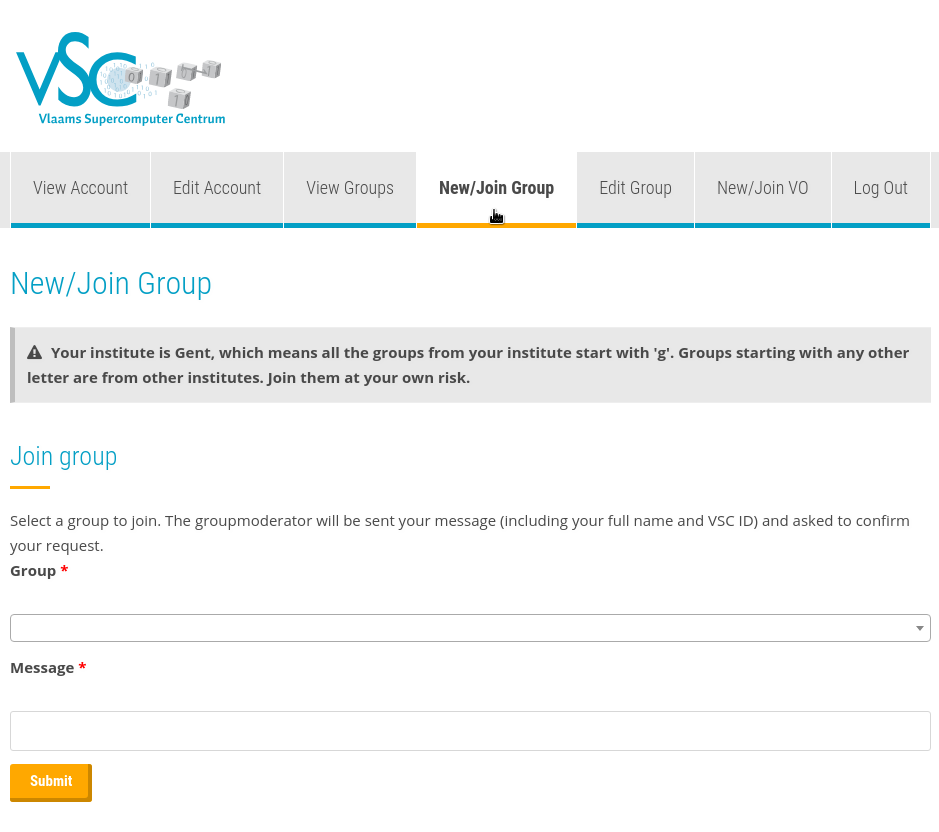
\includegraphics[width=\textwidth]{ch6-group-join}
\end{figure}\label{fig:group-join}

\subsection{Creating a new group}

\begin{enumerate}
    \item Go to \url{https://account.vscentrum.be/django/group/new} and scroll down
        to the section ``Request new group''. This should look something like
        \autoref{fig:group-new}.
    \item Fill out the group name. This cannot contain spaces.
    \item Put a description of your group in the ``Info'' field.
    \item You will now be a member and moderator of your newly created group.
\end{enumerate}

\begin{figure}[!htbp]
  \caption{Creating a new group.}
  \centering
    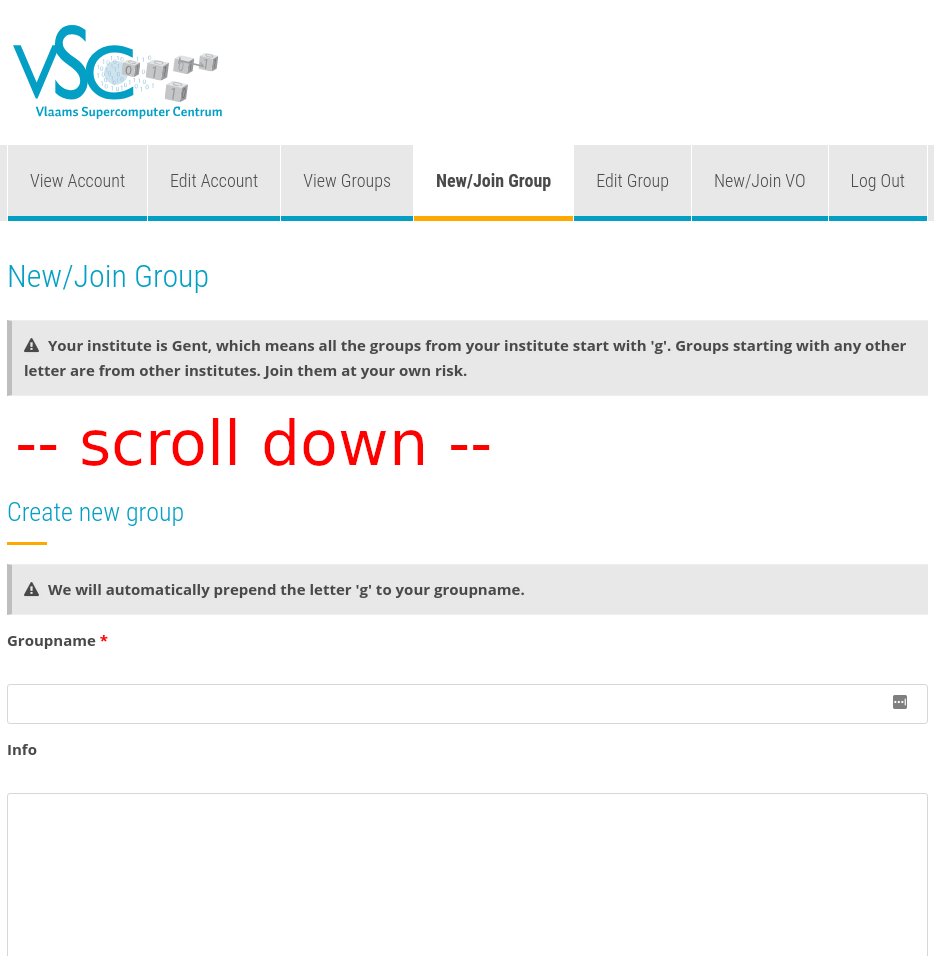
\includegraphics[width=\textwidth]{ch6-group-new}
\end{figure}\label{fig:group-new}

\subsection{Managing a group}

Group moderators can go to \url{https://account.vscentrum.be/django/group/edit} to
manage their group (see \autoref{fig:group-edit}). Moderators can invite and remove members. They can also promote
other members to moderator and remove other moderators.

\begin{figure}[!htbp]
  \caption{Creating a new group.}
  \centering
    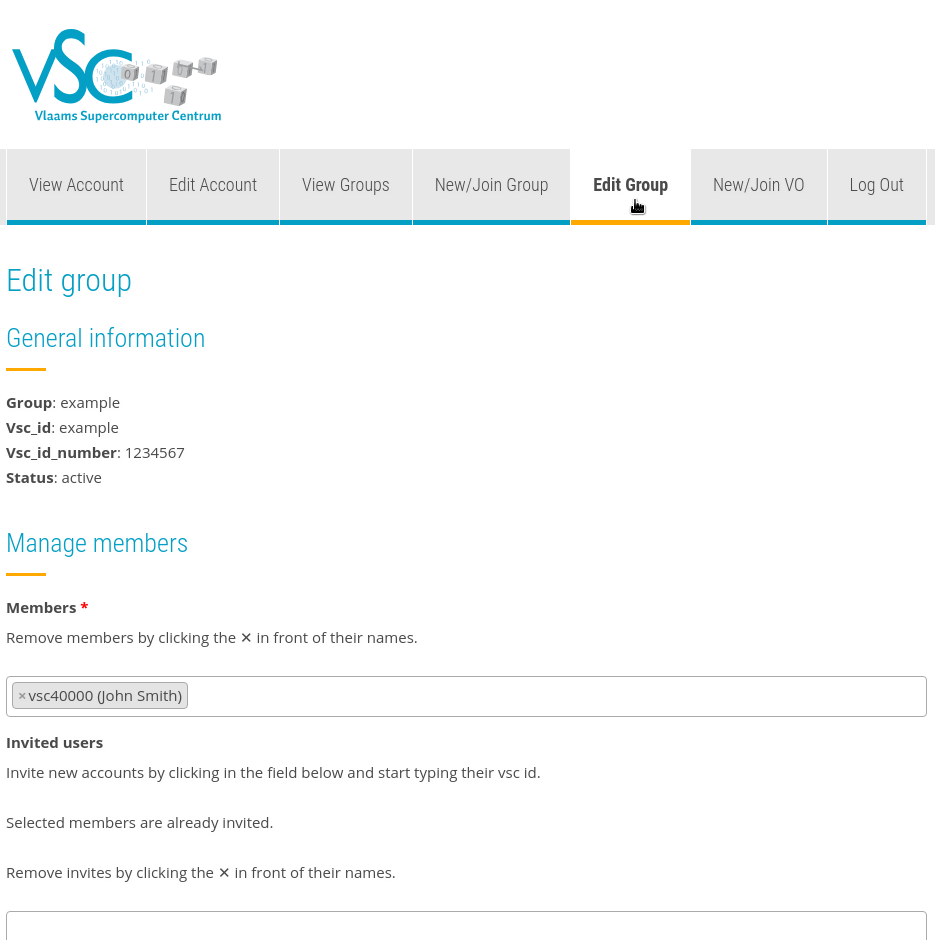
\includegraphics[width=\textwidth]{ch6-group-edit}
\end{figure}\label{fig:group-edit}

% virtual organisations are only used in Ghent (for now)
\ifgent
\section{Virtual Organisations}
\label{sec:virtual-organisations}

A Virtual Organisation (VO) is a special type of group. You can only be a member
of one single VO at a time (or not be in a VO at all).
Being in a VO allows for larger storage quota to be obtained
(but these requests should be well-motivated).

\subsection{Joining an existing VO}

\begin{enumerate}
    \item Get the VO id of the research group you belong to (this id is formed by
        the letters \lstinline|gvo|, followed by 5 digits).
    \item Go to \url{https://account.vscentrum.be/django/vo/join} and fill in the
        section named ``Join VO''. You will be asked to fill in the VO id and a message for
        the moderator of the VO, where you identify yourself. This should look something
        like \autoref{fig:VO-join}.
    \item After clicking the submit button, a message will be sent to the moderator
    of the VO, who will either approve or deny the request.
\end{enumerate}



\begin{figure}[!htbp]
  \caption{Joining a VO.}
  \centering
    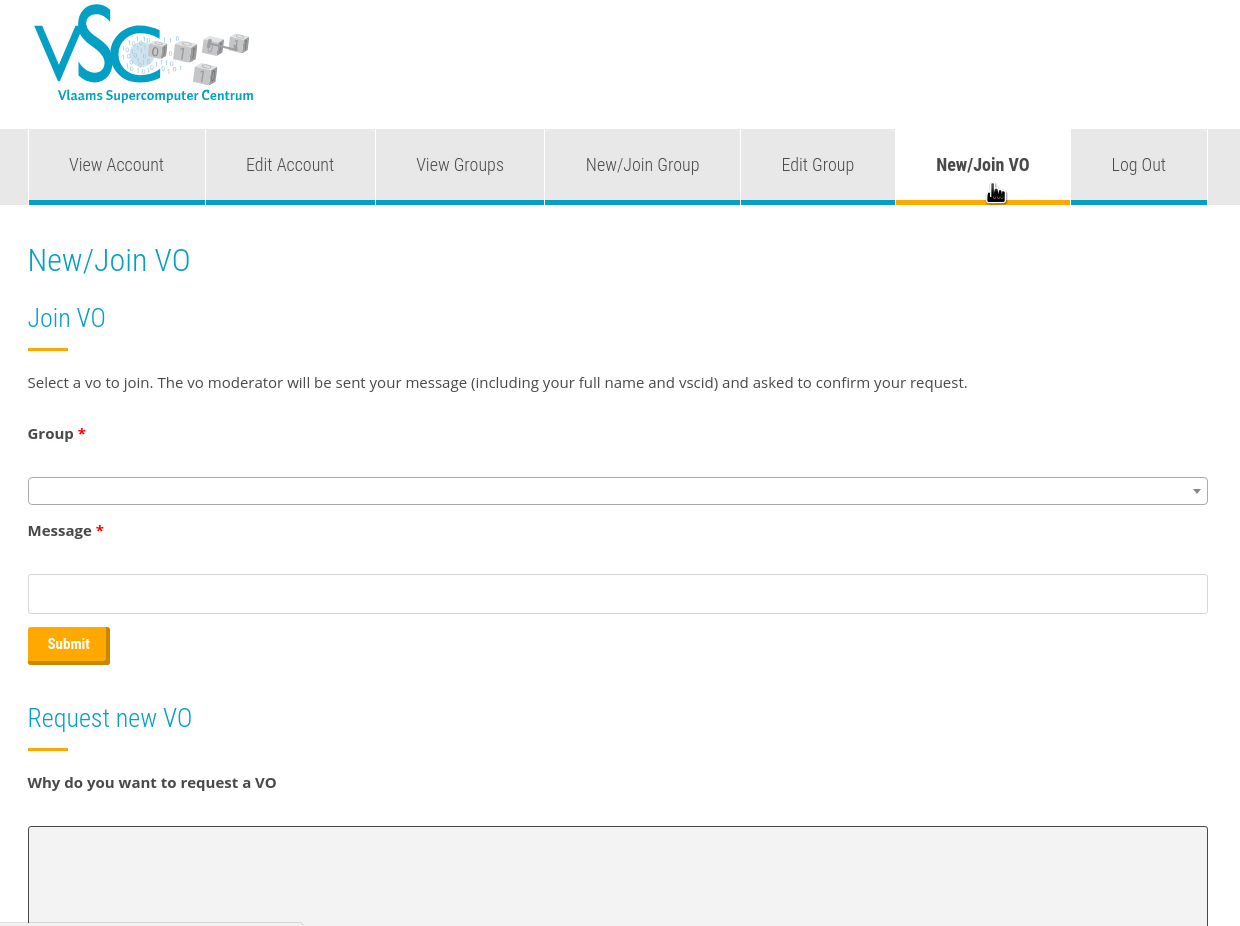
\includegraphics[width=\textwidth]{ch6-VO-join}
\end{figure}\label{fig:VO-join}

\subsection{Creating a new VO}

\begin{enumerate}
    \item Go to \url{https://account.vscentrum.be/django/vo/new} and scroll down
        to the section ``Request new VO''. This should look something like
        \autoref{fig:VO-new}.
    \item Fill why you want to request a VO.
    \item Fill out the both the internal and public VO name. These cannot contain
        spaces, and should be 8-10 characters long. For example, \lstinline|genome25| is
        a valid VO name.
    \item Fill out the rest of the form and press submit. This will send a message
        to the \hpc administrators, who will then either approve or deny the request.
    \item If the request is approved, you will now be a member and moderator of your
        newly created VO.
\end{enumerate}

\begin{figure}[!htbp]
  \caption{Creating a new VO.}
  \centering
    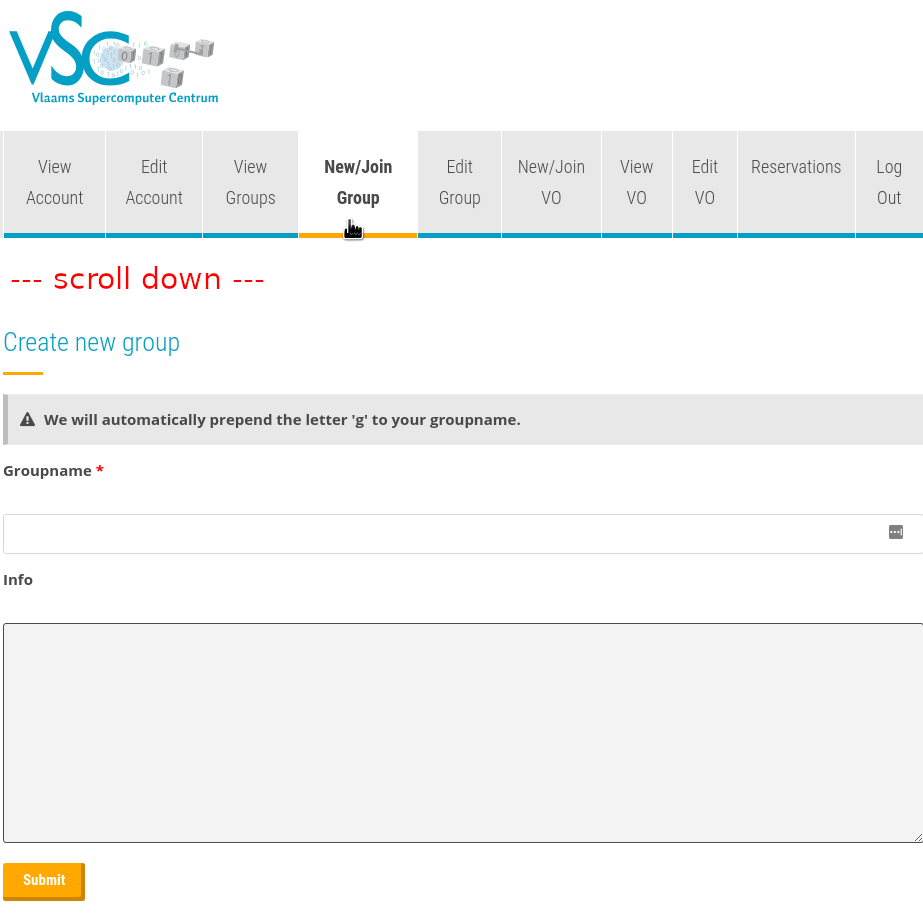
\includegraphics[width=\textwidth]{ch6-VO-new}
\end{figure}\label{fig:VO-new}

\subsection{Requesting more storage space}
\label{subsec:requesting-more-storage-space}

If you're a moderator of a VO, you can request additional quota for the VO and
its members.

\begin{enumerate}
    \item Go to \url{https://account.vscentrum.be/django/vo/edit} and scroll down
        to ``Request additional quota''. See \autoref{fig:VO-request-additional-quota} to see how this looks.
    \item Fill out how much \emph{additional} storage you want. In the screenshot below,
        we're asking for 500 GiB extra space for \lstinline|VSC_DATA|, and for 1 TiB extra
        space on \lstinline|VSC_SCRATCH_KYUKON|.
    \item Add a comment explaining why you need additional storage space and submit
        the form.
    \item An \hpc administrator will review your request and approve or deny it.
\end{enumerate}

\begin{figure}[!htbp]
  \caption{Requesting additional quota for the VO and its members.}
  \centering
    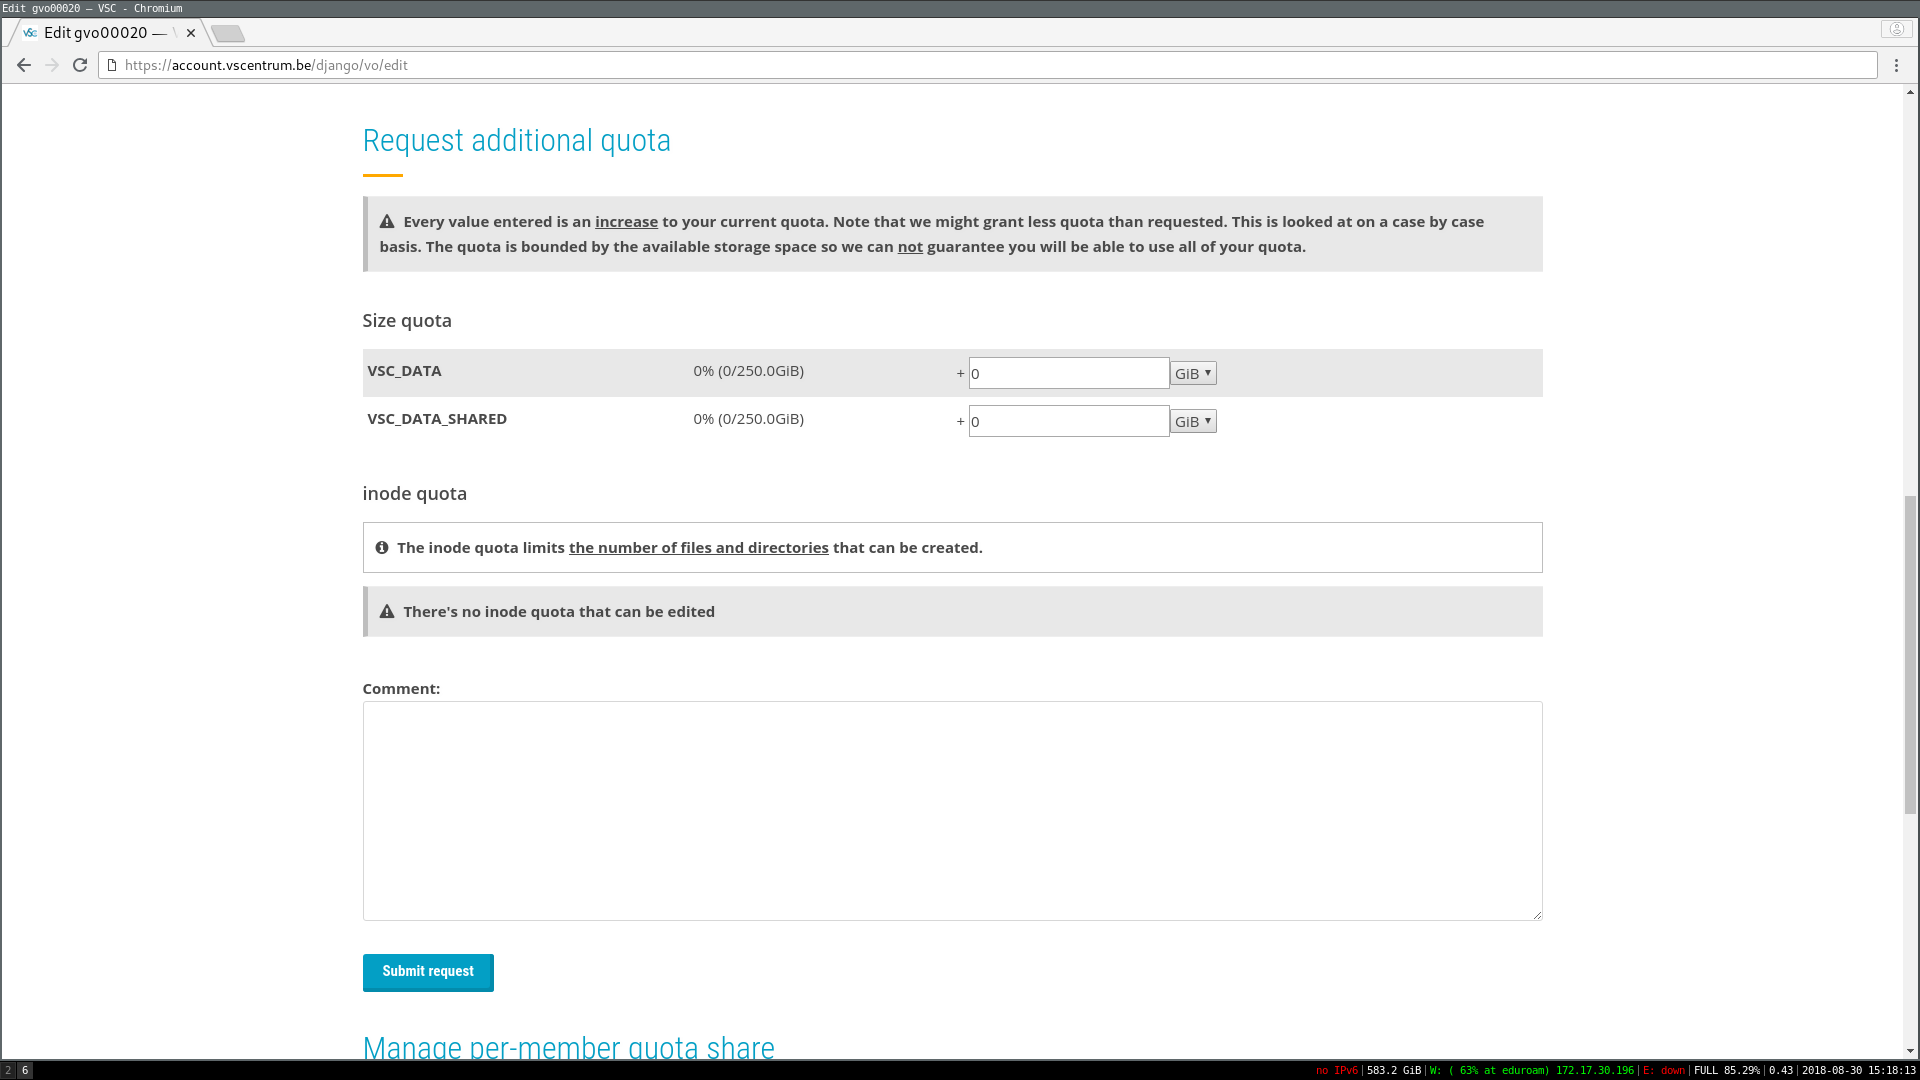
\includegraphics[width=\textwidth]{ch6-VO-request-additional-quota}
\end{figure}\label{fig:VO-request-additional-quota}

\subsection{Setting per-member VO quota}

VO moderators can tweak how much of the VO quota each member can use. By default,
this is set to 50\% for each user, but the moderator can change this: it is possible
to give a particular user more than half of the VO quota (for example 80\%), or
significantly less (for example 10\%).

Note that the total percentage can be above 100\%: the percentages the moderator
allocates per user are \emph{the maximum percentages} of storage users can use.

\begin{enumerate}
    \item Go to \url{https://account.vscentrum.be/django/vo/edit} and scroll down
        to ``Manage per-member quota share''. See \autoref{fig:VO-per-member-storage} to see how this looks.
    \item Fill out how much percent of the space you want each user to be able to use.
        Note that the total can be above 100\%. In the screenshot below, there are
        four users. Alice and Bob can use up to 50\% of the space, Carl
        can use up to 75\% of the space, and Dave can only use 10\% of the space.
        So in total, 185\% of the space has been assigned, but of course only
        100\% can actually be used.
\end{enumerate}

\begin{figure}[!htbp]
  \caption{Setting per-member quota.}
  \centering
    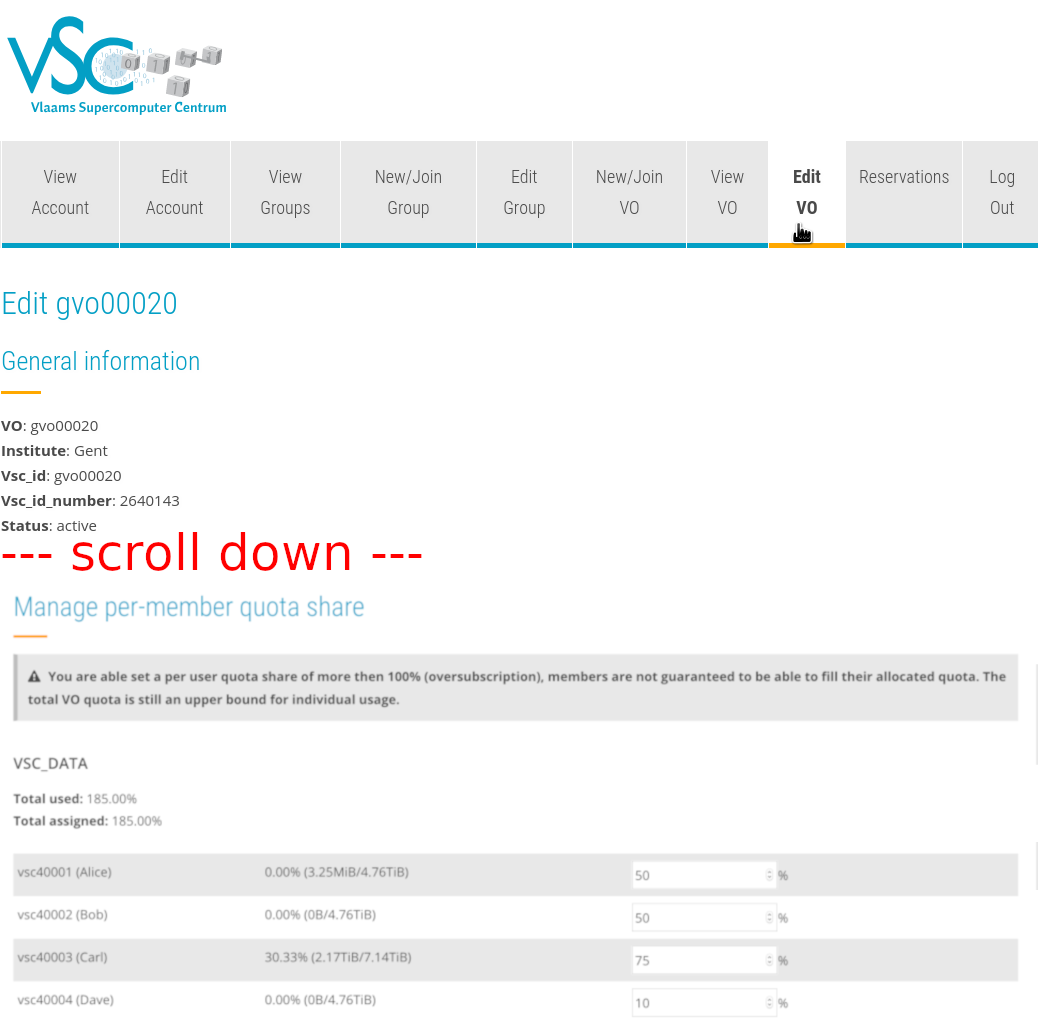
\includegraphics[width=\textwidth]{ch6-VO-per-member-storage}
\end{figure}\label{fig:VO-per-member-storage}

\subsection{VO directories}
\label{subsec:vo-directories}

When you're a member of a VO, there will be some additional directories
on each of the shared filesystems available:

\begin{description}
    \item[VO scratch (\texttt{\$VSC\_SCRATCH\_VO})]
        A directory on the shared \emph{scratch} filesystem shared by the members of your
        VO, where additional storage quota can be provided (see \autoref{subsec:requesting-more-storage-space}).
        You can use this as an alternative to your personal \lstinline|$VSC_SCRATCH|
        directory (see \autoref{subsec:scratch-directory}).

    \item[VO data (\texttt{\$VSC\_DATA\_VO})]
        A directory on the shared \emph{data} filesystem shared by the members of your
        VO, where additional storage quota can be provided (see \autoref{subsec:requesting-more-storage-space}).
        You can use this as an alternative to your personal \lstinline|$VSC_DATA|
        directory (see \autoref{subsec:data-directory}).

\end{description}

If you put \lstinline|_USER| after each of these variable names, you can see your
personal folder in these filesystems. For example: \lstinline|$VSC_DATA_VO_USER|
is your personal folder in your VO data filesystem (this is equivalent to
\lstinline|$VSC_DATA_VO/$USER|), and analogous for \lstinline|$VSC_SCRATCH_VO_USER|.

\fi
